\documentclass[11pt]{article}
\usepackage[utf8]{inputenc}
\usepackage[T1]{fontenc}
\usepackage{amsmath}
\usepackage{amsfonts}
\usepackage{amssymb}
\usepackage[version=4]{mhchem}
\usepackage{stmaryrd}
\usepackage{graphicx}
\usepackage[export]{adjustbox}
\graphicspath{ {./images/} }

\begin{document}
The Three Equity Strategies

This lesson discusses the three major types of equity hedge funds: short-bias funds, equity long/short funds, and equity market-neutral funds. Each of these discussions is framed in the context of the CAPM. The CAPM is used for simplicity as a well-known model with only one factor. The concepts could also be demonstrated with multiple factor models of risk and return but would involve more complexity in mathematical examples.

\section*{Mechanics of Short Selling}
The main factor separating most equity hedge fund managers from traditional equity managers is the use of short selling. The basics of short selling were discussed in Session 5.3, Event-Driven and Relative Value Hedge Funds, in the context of convertible bond arbitrage.

The mechanics of short selling are quite distinct, and short selling requires special skills and risk management techniques. Given the importance of short selling in equity hedge fund strategies, let's explore how the mechanics and risks of short positions differ from those of long positions. Theoretically, a short position can lead to unlimited losses. When an investor purchases a $\$ 100$ stock, the worst loss that can occur is $\$ 100$ if the stock falls to zero. But when an investor short sells a stock at $\$ 100$, there is virtually no limit to how high the stock can go and how large the loss can become. Conversely, long positions can lead to unlimited profits because there is no limit to how high a stock price can go. Short positions can generate only limited profits because the stock price cannot fall below zero. Thus, short selling offers an unattractive profile of limited profit potential and unlimited loss potential, the opposite of long positions.

Short selling also raises potential liquidity problems, because the lender of the security demands collateral to protect its loan. A long/short equity manager can typically post long positions as collateral on the short positions. However, suppose a long/short manager has two investments, A and B, and suppose she holds a long position of $\$ 100$ in $A$ and a short position of $\$ 100$ in $B$. She posts the long position as collateral for the security loan. Now suppose that both positions go against her by $10 \%$ in one day. Thus, stock A goes down from $\$ 100$ to $\$ 90$, and stock B goes up from $\$ 100$ to $\$ 110$. The manager now needs to have $\$ 110$ in collateral to cover the short position that has risen to $\$ 110$. But the collateral that was posted-stock $A-$ has fallen to $\$ 90$. A highly leveraged fund manager may eventually be forced to liquidate the long positions that have fallen in value and buy back the stocks that have risen and that underlie the short positions-both of which may generate poor price executions in a period of illiquidity.

Another potentially huge complexity from short selling is that the lender of the security may demand that the shares be returned. Most securities are lent on a shortterm basis, with the lender retaining the right to demand that the shares be returned at any moment. Usually when this happens, the broker simply arranges for another securities lender to loan shares so that the short seller maintains a seamless exposure.

But especially in times of overall market turbulence, or in times of turbulence for a particular stock, the shares become difficult to borrow. In those cases, the short seller may be forced to cover the position. This means that the short seller must purchase the shares in the market so that they can be returned to the securities lender. The short seller is therefore forced to close his position during a period of turbulence rather than at a time of his choosing. Note that an investor with a long position in a stock does not face this risk. The short seller's potential problem of being forced to liquidate a position is especially acute during a short squeeze, discussed in Session, The Environment of Alternative Investments.

Calculating the total return from short selling is a little more complex than calculating the total return of long positions. For long positions, the return on a stock is the percentage capital gain or loss expressed as a proportion of price, plus any dividends received also expressed as a percentage of price. When the short seller provides cash as collateral for borrowing shares (including the posting of the proceeds from the short sale), the seller typically receives interest in the form of a rebate on the collateral from the securities lender.

The returns on a short position involve three major components: (1) capital gain or loss, (2) dividends, and (3) the short stock rebate on the collateral.

\section*{The Basics of Short-Bias Funds}
Managers of short-bias hedge funds may be distinguished from equity long/short managers in that they generally maintain a net short exposure to the stock market. However, short-selling hedge funds tend to adjust their short exposures in an effort to time markets. That is, they trim their short positions when they anticipate that the stock market is more likely to rise, and they go fully short when they anticipate that the stock market is more likely to decline.

Short-bias fund managers face a difficult challenge: Equity markets typically rise over time due to the equity risk premium, so short-bias funds should be expected to rise very little or perhaps even decline in an efficient market. To earn consistent profits as a short-bias manager, the manager must identify stocks that generally decline in value, even though the overall stock market generally rises.

In theory, short-bias funds should be evaluated on performance relative to their negative systematic risk. Thus, negative performance should be tolerated or even praised if the fund's beta is substantially negative, if equity markets have risen, and if the negative performance is minimal. The reason that low or even negative returns from short-bias funds should be tolerated is that short-selling strategies provide good downside protection for bear markets. Short-bias funds can be included in a portfolio with a positive beta for the hedging and protection against downside risk, but short-bias funds should not be the focal point for generating excess returns.

For example, consider a world in which the CAPM holds, the expected return of the market portfolio is $12 \%$, and the riskless rate is $2 \%$. Assume that a long-only fund with a beta of 1.0 offers an expected return of $14 \%$, and a short-bias fund with a beta of -1.0 offers an expected return of $-4 \%$. Using the CAPM, the ex ante alpha of the long-only fund is $2 \%$, and the ex ante alpha of the short-bias fund is $4 \%$. Should an asset allocator consider the short-bias fund to be a valuable addition to a portfolio? The answer is yes. Consider a portfolio invested 50\% in the long-only fund and 50\% in the short-bias fund. This portfolio of two funds would have a net beta exposure of zero. However, the expected return of the combination would be $5 \%$ (found as $50 \% \times 14 \%$ for the long-only fund, and $50 \% \times-4 \%$ for the short-bias fund). With zero systematic risk, the ex ante alpha of the combination is its expected return in excess of the riskless rate: $3 \%$. The computation of the ex ante alpha is confirmed by summing $50 \%$ of the ex ante alpha of the long-only fund $(50 \% \times 2 \%)$ and $50 \%$ of the ex ante alpha of the short-bias fund $(50 \% \times 4 \%)$.

This example shows that, in theory, a negative expected return to a short-bias fund may be acceptable if the fund offers a sufficiently negative beta to hedge the positive beta of other funds. The focus in evaluating a short-bias fund should be its returns relative to the systematic risk, not the fund's absolute returns.

Finally, there are reputational and regulatory risks to short selling that do not exist for funds that establish only long positions. During the 2008 financial crisis some countries restricted short selling altogether, while others restricted short sales in particular stocks, such as the shares of firms in the financial sector. Hedge funds that require the short sales of stock, such as short-bias funds, convertible bond funds, and merger arbitrage funds, may not be able to properly implement their strategies during times of short sale restrictions. Specifically, without short selling being allowed, some hedge funds may have a greater than desired net long exposure to the underlying market. Regulations may also have or institute an uptick rule that permits short sellers to enter a short sale only at a price that is equal to or higher than the previous transaction price of the stock. The goal of regulators is to prevent short sales from directly causing a downward spiral in the price of a stock by completing executions at lower and lower prices. Short sellers may also be politically unpopular, as they may be perceived to revel in a company's failure, or even to be the cause of a sharp decline in a company's stock price.

\section*{Key Observations Regarding Returns of Short-Bias Funds}
Short bias fund returns are observed from January of 2005 to December of 2021 for a total of 204 observations. Statistical Summary of Returns provides univariate return statistics and partial autocorrelations of returns in the top panel, and a histogram of returns in the bottom panel.

\begin{center}
\begin{tabular}{lcc}
\hline
Index (Jan. 2005-Dec. 2021) & \begin{tabular}{c}
HFRX Equity Hedge: \\
Short Bias \\
\end{tabular} & \begin{tabular}{c}
MSCI World \\
Equity \\
\end{tabular} \\
\hline
Annualized Arithmetic Mean & $-8.5 \%$ & $9.1 \%$ \\
Annualized Standard Deviation & $16.4 \%$ & $15.3 \%$ \\
Annualized Semivolatility & $13.1 \%$ & $12.3 \%$ \\
Annualized Median & $-9.1 \%$ & $16.0 \%$ \\
Skewness & -0.5 & -0.8 \\
Excess Kurtosis & 4.6 & 2.3 \\
Sharpe Ratio & -0.7 & 0.4 \\
Sortino Ratio & -0.8 & 0.5 \\
Annualized Geometric mean & $-9.8 \%$ & $8.0 \%$ \\
First-Order Autocorrelation & 0.1 & 0.1 \\
Annualized Standard Deviation & $15.3 \%$ & $14.9 \%$ \\
(Adjusted for Autocorrelation) & $17.9 \%$ & $12.8 \%$ \\
Maximum & $-22.9 \%$ & $-19.0 \%$ \\
Minimum & $-87.4 \%$ & $-54.0 \%$ \\
\hline
\end{tabular}
\end{center}

\begin{center}
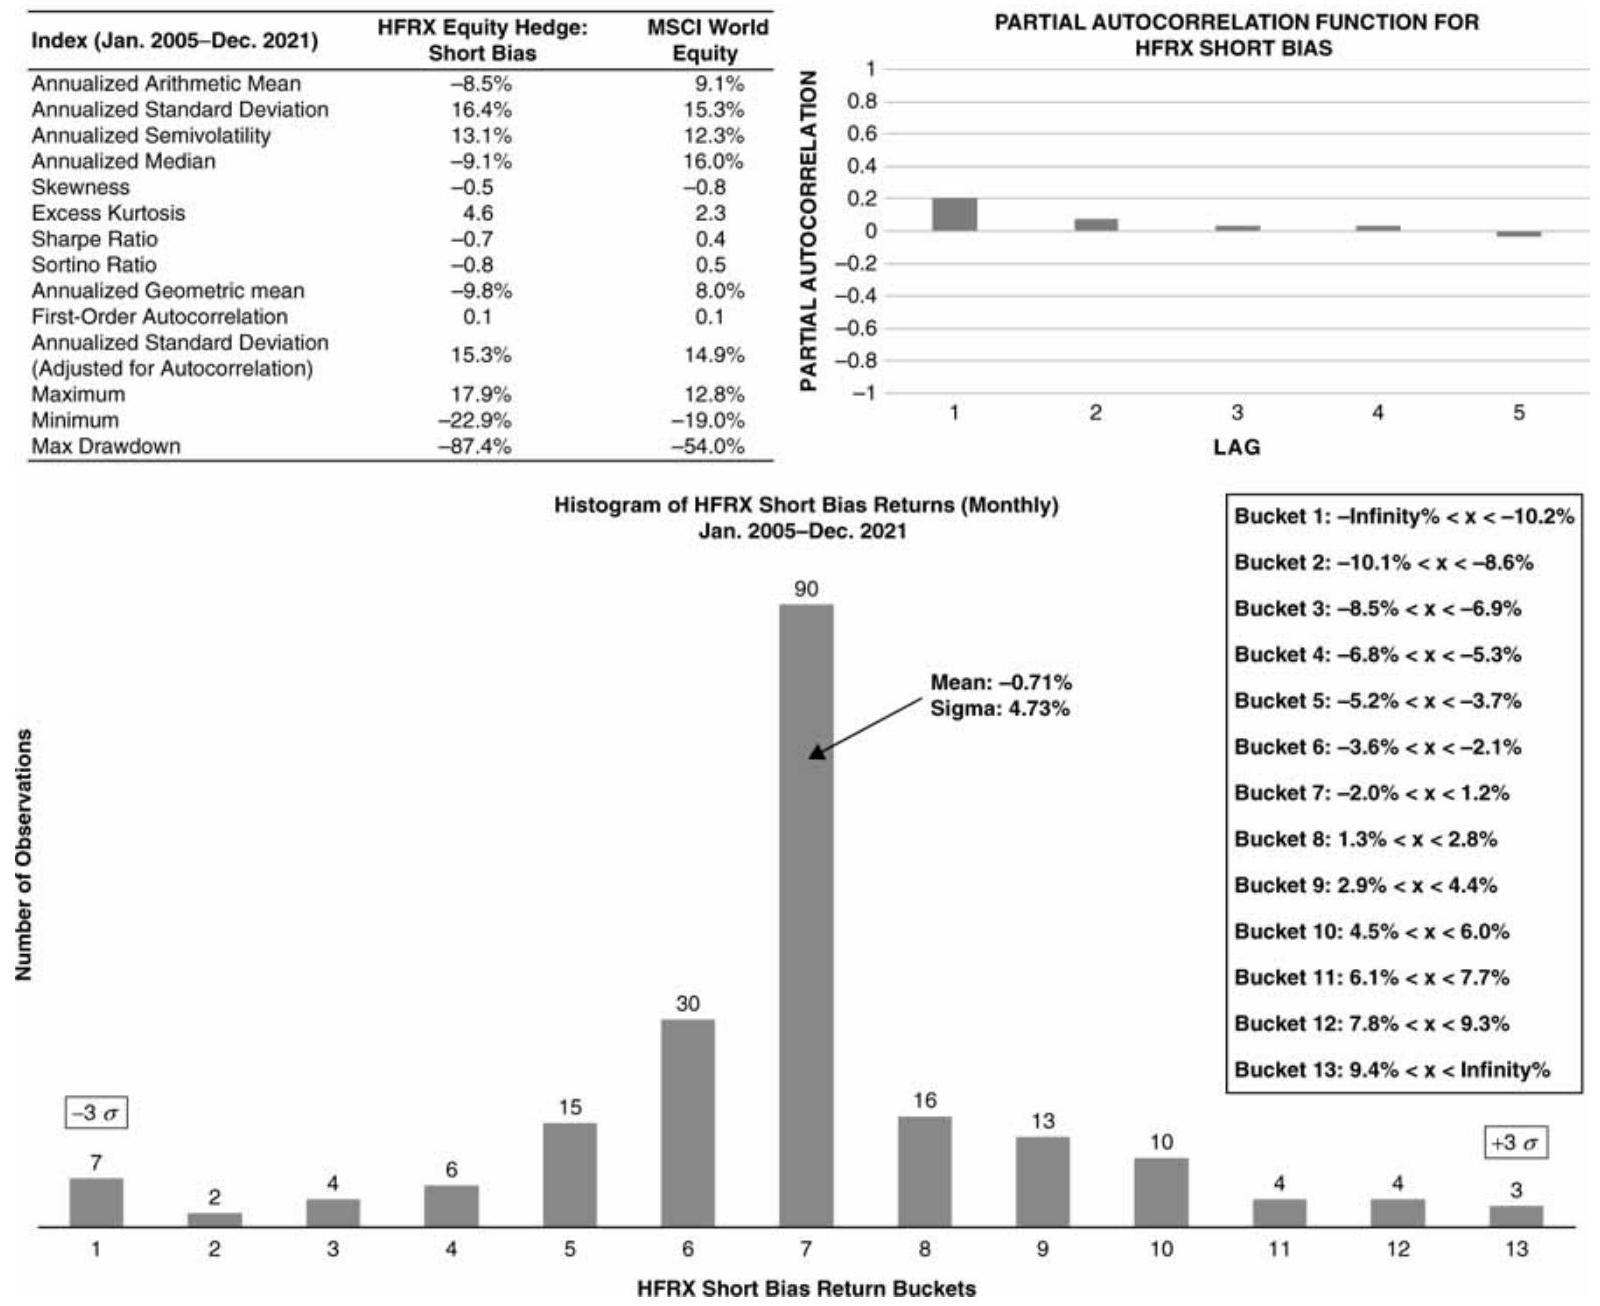
\includegraphics[max width=\textwidth]{2024_04_09_92122b5eb0776b473e03g-3}
\end{center}

\section*{Statistical Summary of Returns}
Key observations on long-short equity returns that are consistent with economic reasoning (and are consistent with and driven by the use of appraisals for valuations) are an essential component of knowledge and include the following:

\begin{enumerate}
  \item Short bias historical equity returns averaged annual returns of roughly $-8.8 \%$, which is to be expected given the average returns of world equities of roughly $+8.4 \%$.

  \item Short bias historical equity returns indicated similar volatility than that of world equities.

  \item Returns had similar skew and excess kurtosis as world equities.

  \item Maximum drawdown was much higher than that of world equities.

  \item Returns had very slight but consistently positive first through fourth order partial autocorrelations.

\end{enumerate}

In summary, these short-biased returns exhibited mean returns and risk levels expected from being the opposite exposure of an index of long world equities.

\section*{The Basics of Equity Long/Short Funds}
Equity long/short managers build their portfolios by combining a core group of long stock positions with short sales of stock, or bearish positions in stock index options and futures. Their net market exposure of long positions minus short positions tends to have a positive bias. That is, equity long/short managers tend to be long market exposure by typically having a larger long position than short position.

As a simplified example, consider a hedge fund manager who at the beginning of 2008 held $150 \%$ of the portfolio value in a long position in the SPDR XME, an exchange-traded fund (ETF) that passively replicates exposure to the metals and mining sector of the S\&P 500. Simultaneously, the hedge fund manager established a short position of $50 \%$ of the portfolio value in the SPDR XLF, an ETF that passively replicates exposure to the financial sector of the S\&P 500. Assume that the relevant market index is the S\&P 500, that the estimated beta of the XME is 0.99 , and that the estimated beta of the XLF is 0.98 . Therefore, the weighted average beta of this equity long/short portfolio is $(1.5 \times 0.99)-(0.5 \times 0.98)=0.995$.

This long/short equity portfolio has approximately the same systematic risk as the S\&P 500. In the period from January 2008 through August 2008, the return on the S\&P 500 was $-13.64 \%$, and the risk-free rate was about $2.25 \%$. Given the realized return on the market portfolio and the beta of the hedge fund, the realized return on this portfolio, ignoring idiosyncratic risk and using the CAPM, should be as follows:

$$
\text { Return }=2.25 \%+0.995(-13.6 \%-2.25 \%)=-13.52 \%
$$

However, from January to August 2008, the return on the XLF was -33\%, and the return on the XME was $+23 \%$. This portfolio, with a beta of approximately one, would have earned the following return, ignoring fees and transaction costs:

$$
(1.5 \times 23 \%)+(-0.5 \times-33 \%)=51 \%
$$

This is a much higher return than that predicted by the CAPM. The ability to go both long and short in the market is a powerful tool for magnifying idiosyncratic risk without necessarily magnifying systematic risk. Higher idiosyncratic risks offer skilled managers greater breadth and an opportunity to generate higher ex ante alpha. The long/short nature of the portfolio can be misleading with respect to the risk exposure. This manager appears to have risk similar to that of the S\&P 500, and an investor might conclude that returns similar to those of the S\&P 500 will be realized. However, what the hedge fund manager has done is make two idiosyncratic bets: that financial stocks will underperform and that metals and mining stocks will outperform. Even though the fund has market exposure similar to that of the index, the extreme industry exposures can create substantial risk.

Many hedge fund managers build concentrated positions in an attempt to take advantage of forecasted deviations of expected returns from the predictions of the CAPM. The important question is whether hedge fund managers, with their flexible mandates and strong incentives, are able to identify and to take advantage of mispricings.

Equity long/short hedge funds essentially come in two varieties: quantitative or fundamental. Quantitative managers use precise, objective models to identify trading opportunities. These models are often focused on technical analysis but may use fundamental measures in addition to or instead of technical indicators.

Fundamental equity long/short hedge funds conduct fundamental analysis on a company's business prospects, including its competition and the current economic environment. These managers may visit with management, talk with Wall Street analysts, contact customers and competitors, and essentially conduct bottom-up analysis. A difference between these hedge funds and long-only managers is that hedge fund managers can short the stocks that they predict will be poor performers. In addition, they may leverage their positions.

Fundamental equity long/short hedge funds may invest broadly or in one economic sector. Equity long/short managers who focus on one sector are called sector hedge funds. For example, sector hedge funds are equity long/short managers who specialize in a specific sector, such as biotechnology, health care, or natural resources. These are typically fundamental stock pickers who have considerable knowledge and experience in analyzing companies in a specialized sector of the economy. They go both long and short, using their fundamental information advantage to find both excellent and poorly performing companies in that sector. Typically, they have a long beta exposure-sometimes a very long beta exposure-with only a few short positions offsetting many long positions.

\section*{Key Observations Regarding Historical Returns for Equity Long/Short Funds}
Equity long-short fund returns are observed from January of 2000 to December of 2021 for a total of 264 observations. Statistical Summary of Returns provides univariate return statistics and partial autocorrelations of returns in the top panels, and histograms of returns in the bottom panels.

\begin{center}
\begin{tabular}{lcc}
\hline
Index (Jan. 2000-Dec. 2021) & \begin{tabular}{c}
Credit Suisse Long/Short \\
Equity \\
\end{tabular} & \begin{tabular}{c}
MSCI World \\
Equity \\
\end{tabular} \\
\hline
Annualized Arithmetic Mean & $5.8 \%$ & $6.8 \%$ \\
Annualized Standard Deviation & $7.9 \%$ & $15.4 \%$ \\
Annualized Semivolatility & $5.9 \%$ & $11.8 \%$ \\
Annualized Median & $6.4 \%$ & $15.1 \%$ \\
Skewness & -0.3 & -0.6 \\
Excess Kurtosis & 2.9 & 1.6 \\
Sharpe Ratio & 0.4 & 0.3 \\
Sortino Ratio & 0.6 & 0.4 \\
Annualized Geometric mean & $5.5 \%$ & $5.6 \%$ \\
First-Order Autocorrelation & 0.1 & 0.1 \\
Annualized Standard Deviation & $8.6 \%$ & $17.0 \%$ \\
(Adjusted for Autocorrelation) & $11.1 \%$ & $12.8 \%$ \\
Maximum & $-7.8 \%$ & $-19.0 \%$ \\
Minimum & $-22.0 \%$ & $-54.0 \%$ \\
Max Drawdown &  &  \\
\hline
 & HFRI Equity & MSCI World \\
\hline
Hedge (Total) & Equity &  \\
\hline
Annualized Arithmetic Mean (Jan. 2000-Dec. 2021) & $6.1 \%$ & $6.8 \%$ \\
Annualized Standard Deviation & $8.7 \%$ & $15.4 \%$ \\
Annualized Semivolatility & $6.7 \%$ & $11.8 \%$ \\
Annualized Median & $9.1 \%$ & $15.1 \%$ \\
Skewness & -0.5 & -0.6 \\
Excess Kurtosis & 3.0 & 1.6 \\
Sharpe Ratio & -0.3 & 0.3 \\
Sortino Ratio & -0.4 & 0.4 \\
Annualized Geometric mean & $5.7 \%$ & $5.6 \%$ \\
First-Order Autocorrelation & 0.2 & 0.1 \\
Annualized Standard Deviation & $10.3 \%$ & $17.0 \%$ \\
(Adjusted for Autocorrelation) & $10.0 \%$ & $12.8 \%$ \\
Maximum & $-10.9 \%$ & $-19.0 \%$ \\
Minimum & $-30.6 \%$ & $-54.0 \%$ \\
Max Drawdown &  &  \\
\end{tabular}
\end{center}

PARTIAL AUTOCORRELATION FUNCTION FOR CREDIT SUISSE LONG/SHORT EQUITY

\begin{center}
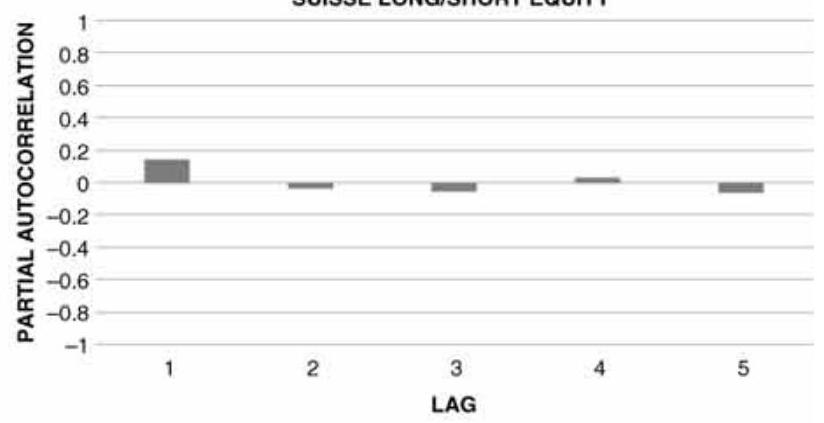
\includegraphics[max width=\textwidth]{2024_04_09_92122b5eb0776b473e03g-5}
\end{center}

PARTIAL AUTOCORRELATION FUNCTION FOR HFRI EQUITY HEDGE (TOTAL)

\begin{center}
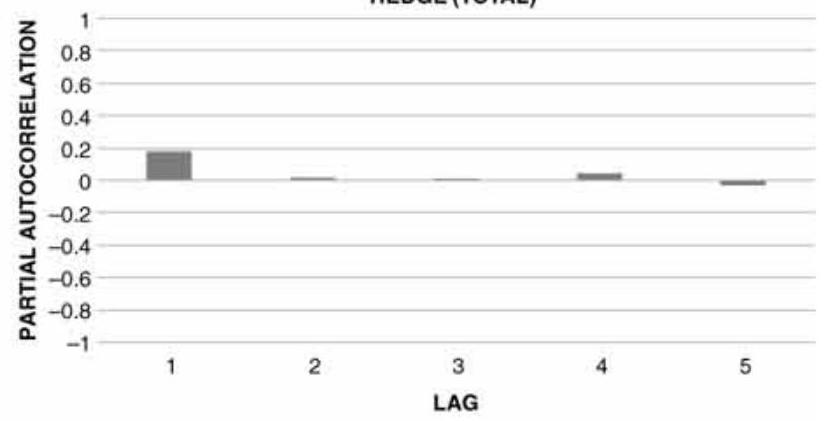
\includegraphics[max width=\textwidth]{2024_04_09_92122b5eb0776b473e03g-5(1)}
\end{center}

Histogram of Credit Suisse: Long/Short Equity (Monthly) Jan. 2000-Dec. 2021

\begin{center}
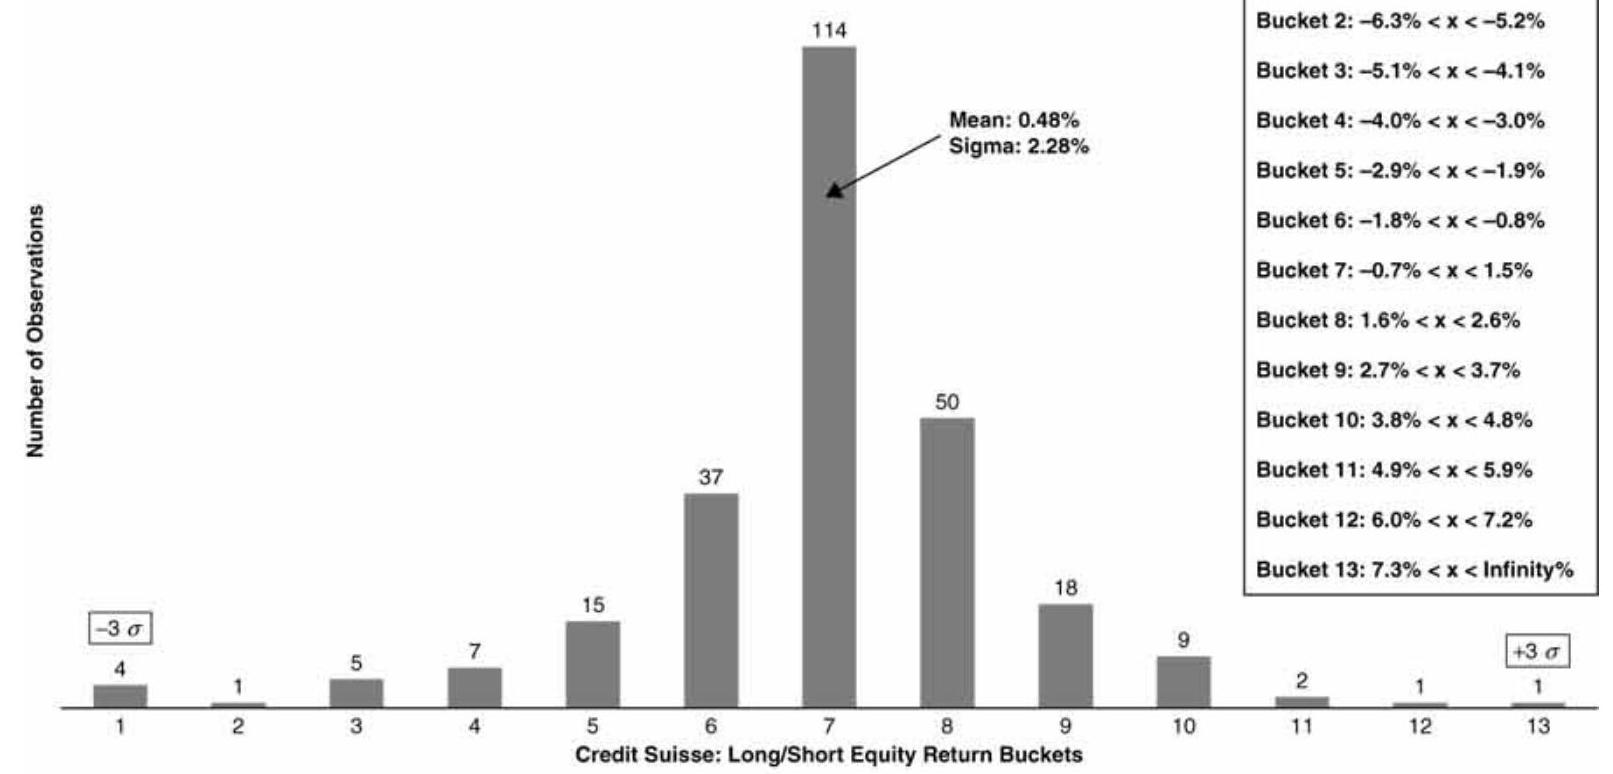
\includegraphics[max width=\textwidth]{2024_04_09_92122b5eb0776b473e03g-5(2)}
\end{center}

Histogram of HFRI Equity Hedge (Total) Returns (Monthly) Jan. 2000-Dec. 2021

\begin{center}
\begin{tabular}{l}
Bucket 1: -Infinity $\%<x<-6.8 \%$ \\
Bucket 2: $-6.7 \%<x<-5.6 \%$ \\
Bucket 3: $-5.5 \%<x<-4.4 \%$ \\
Bucket 4: $-4.3 \%<x<-3.3 \%$ \\
Bucket 5: -3.2\%<x<-2.1\% \\
Bucket 6: -2.0\%<x<-0.9\% \\
Bucket 7:-0.8\%<x<1.5\% \\
Bucket 8: 1.6\%<x<2.7\% \\
Bucket 9: 2.8\%<x<3.9\% \\
Bucket 10: $4.0 \%<x<5.0 \%$ \\
Bucket 11: 5.1\% $2<6.2 \%$ \\
Bucket 12: $6.3 \%<x<7.5 \%$ \\
Bucket 13: $7.6 \%<x<$ Infinity $\%$ \\
\hline
\end{tabular}
\end{center}

\section*{Statistical Summary of Returns}
Key observations on long-short equity returns that are consistent with economic reasoning (and are consistent with and driven by the use of appraisals for valuations) are an essential component of knowledge and include the following:

\begin{enumerate}
  \item Long-short historical equity returns indicated roughly half the volatility of world equities.

  \item Long-short returns were symmetrical but with substantially higher excess kurtosis than world equities.

  \item Maximum drawdown was less than half that of world equities.

  \item Returns had slightly positive first-order partial autocorrelations.

\end{enumerate}

In summary, these hedged returns exhibited generally lower risk than a long-only index of world equities, except in the case of excess kurtosis.

\section*{The Basics of Equity Market-Neutral Funds}
Like equity long/short funds, equity market-neutral hedge funds establish both long and short positions in the equity market. The difference is that equity marketneutral funds maintain integrated portfolios that are designed to neutralize equity market risk, bringing beta risk to zero. This generally means a target of being neutral not just to the overall stock market but also across sectors. The idea of equity market-neutral funds is to neutralize market and industry risk and concentrate purely on stock selection in both the long and short positions. Although equity market-neutral fund managers seek alpha through security selection, unlike equity long/short managers, they strive for market neutrality rather than engaging in market timing.

Patton discusses a number of definitions of market neutrality. ${ }^{1}$ Andrew J. Patton (2009), Are "Market-Neutral" Hedge Funds Really Market Neutral? Review of Financial Studies 22 (no. 7): 2295-330. More than 70\% of funds in the merger arbitrage, convertible arbitrage, relative value arbitrage, and equity market-neutral categories are found to be statistically indistinguishable from being market neutral. This is in contrast to the hedge fund strategies commonly known to be directional, in which perhaps half to two-thirds of the funds are shown to have statistically significant directional market exposure. The standard definition of market neutrality is mean neutrality. Mean neutrality is when a fund is shown to have zero beta exposure or correlation to the underlying market index. In other words, when the market experiences a move in one direction, mean-neutral funds are no more likely to move in the same direction as in the opposite direction. In addition, investors may consider whether their hedge fund exhibits variance neutrality. Variance neutrality is when fund returns are uncorrelated to changes in market risk, including extreme risks in crisis market scenarios. The concept of variance neutrality can be extended into other measures of risk, such as value-at-risk neutrality or tail neutrality. Patton found evidence that perhaps one-fourth of funds failed to be independent from market risk.

Some equity market-neutral managers use leverage. But being market beta neutral is not a zero-risk strategy. Consider the years 1998 and 1999, in which some quantitative equity investors were long value stocks and short growth stocks. Even with a zero market beta, substantial losses were experienced when managers were not sector or industry neutral. For example, profits from long positions in retail stocks were not able to overcome losses from the short positions in Internet stocks.

Generally, equity market-neutral managers follow a three-step procedure in their strategy. The first step is to build an initial screen of investable stocks. These are stocks that are traded on the exchanges the manager follows, that have sufficient liquidity to enable the fund to enter and exit positions quickly, and that may be borrowed from the hedge fund manager's prime broker for short positions. Additionally, the hedge fund manager may limit her universe by using other criteria, such as a capitalization segment (e.g., mid-caps). Next, the manager analyzes investable stocks to identify those stocks that are attractive candidates for long positions, in that they are perceived to be underpriced, and those that are attractive candidates for short positions, in that they are perceived to be overpriced. Finally, the portfolio is constructed. The hedge fund manager uses a computer program to identify portfolio weights so as to be neutral to the overall market as well as potentially neutral across sectors.

Most equity market-neutral managers use optimizers to neutralize market and sector exposure. However, more sophisticated optimizers attempt to keep the portfolio neutral to several risk factors, including size, price-to-earnings ratio, book-to-market ratio, leverage, liquidity, and currency sensitivity. The idea is to have no intended or unintended risk exposures that might compromise the portfolio's neutrality.

Because equity market-neutral portfolios are designed to produce returns independent of the market, these strategies are especially sensitive to the manager's or the model's stock-picking skill. Crowded trades, in which hedge funds control a significant portion of the stock's outstanding shares, are a special risk, especially among leveraged managers trading factor models. To the extent that multiple quantitative managers are using similar factor models, many managers have similar positions. If these managers need to liquidate positions rapidly, such as occurred in August 2007, losses may occur as long positions are sold and short positions are covered without regard for market impact.

\section*{Key Observations Regarding Historical Returns of Equity Market-Neutral Funds}
Equity market-neutral returns are observed from January of 2000 to December of 2021 for a total of 264 observations. Statistical Summary of Returns provides univariate return statistics and partial autocorrelations of returns in the top panel, and a histogram of returns in the bottom panel.

\begin{center}
\begin{tabular}{lcc}
\hline
Index (Jan. 2000-Dec. 2021) & \begin{tabular}{c}
HFRI Equity Hedge: Equity MSCI World \\
Market Neutral \\
\end{tabular} & \begin{tabular}{c}
Equity \\
\end{tabular} \\
\hline
Annualized Arithmetic Mean & $3.4 \%$ & $6.8 \%$ \\
Annualized Standard Deviation & $2.8 \%$ & $15.4 \%$ \\
Annualized Semivolatility & $2.2 \%$ & $11.8 \%$ \\
Annualized Median & $3.8 \%$ & $15.1 \%$ \\
Skewness & -0.5 & -0.6 \\
Excess Kurtosis & 2.8 & 1.6 \\
Sharpe Ratio & 0.3 & 0.3 \\
Sortino Ratio & 0.4 & 0.4 \\
Annualized Geometric mean & $3.3 \%$ & $5.6 \%$ \\
First-Order Autocorrelation & 0.1 & 0.1 \\
Annualized Standard Deviation & $3.0 \%$ & $17.0 \%$ \\
(Adjusted for Autocorrelation) & $3.1 \%$ & $12.8 \%$ \\
Maximum & $-2.9 \%$ & $-19.0 \%$ \\
Minimum & $-9.2 \%$ & $-54.0 \%$ \\
Max Drawdown &  &  \\
\end{tabular}
\end{center}

PARTIAL AUTOCORRELATION FUNCTION FOR HFRI EQUITY HEDGE: EQUITY MARKET NEUTRAL

\begin{center}
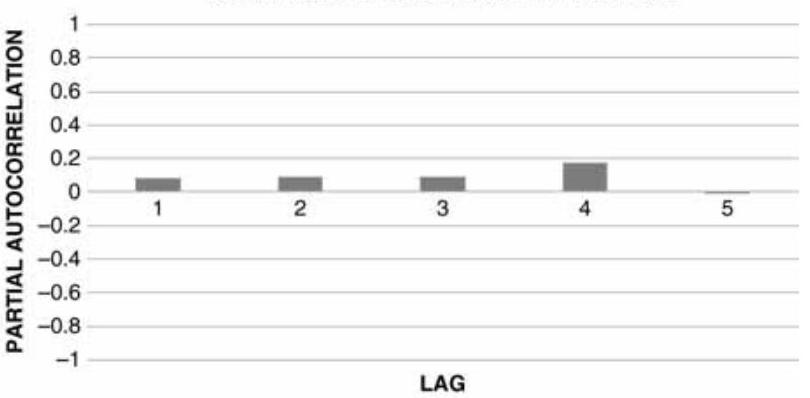
\includegraphics[max width=\textwidth]{2024_04_09_92122b5eb0776b473e03g-7}
\end{center}

Histogram of HFRI Equity Hedge: Equity Market Neutral Returns (Monthly) Jan. 2000-Dec. 2021

\begin{center}
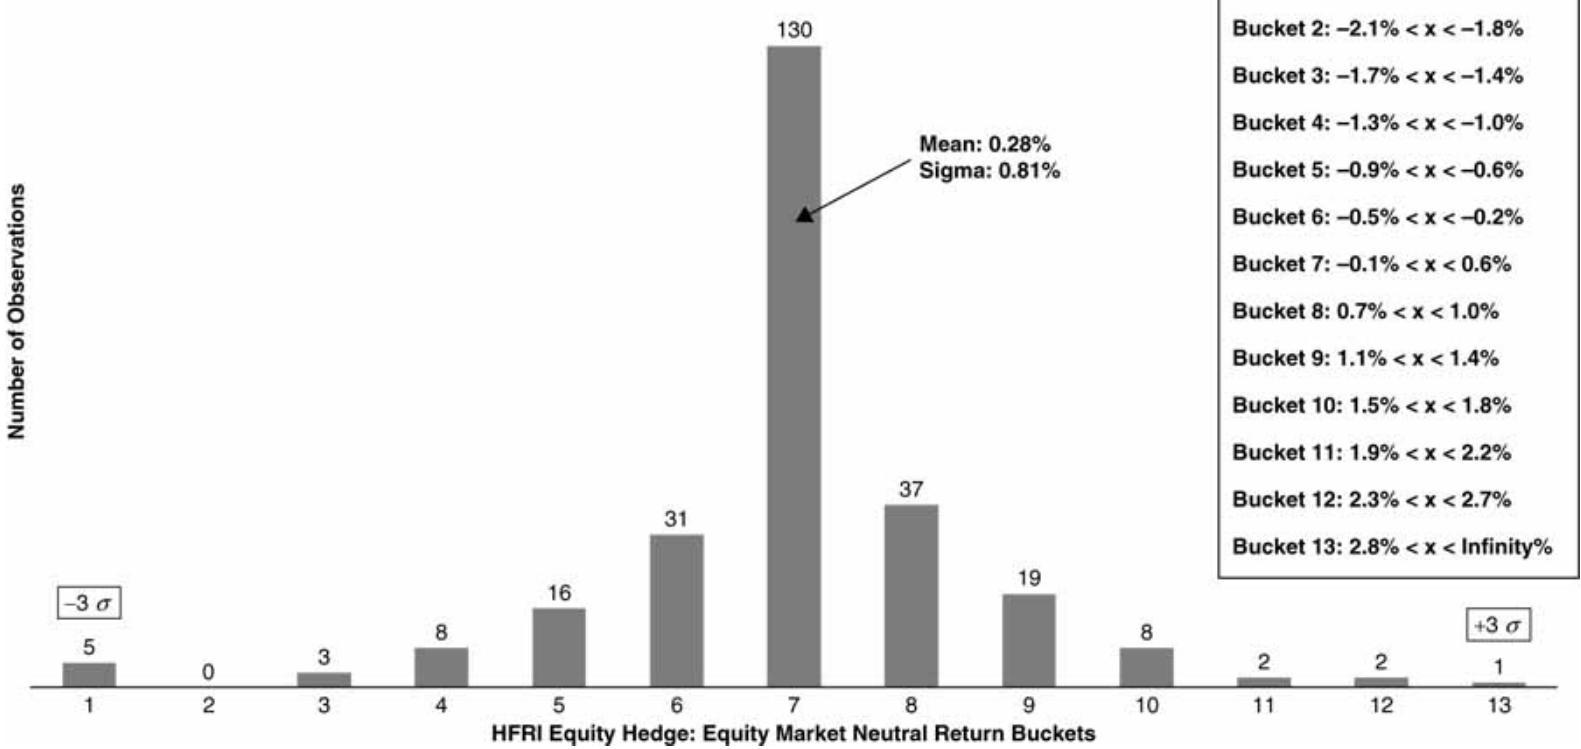
\includegraphics[max width=\textwidth]{2024_04_09_92122b5eb0776b473e03g-7(1)}
\end{center}

\section*{Statistical Summary of Returns}
Key observations on long-short equity returns that are consistent with economic reasoning (and are consistent with and driven by the use of appraisals for valuations) are an essential component of knowledge and include the following:

\begin{enumerate}
  \item Equity market-neutral historical equity returns indicated a mere fifth of the volatility of world equities.

  \item Equity market-neutral returns were roughly symmetrical but exhibited moderately higher excess kurtosis than world equities.

  \item Maximum drawdown was approximately $20 \%$ the size of that of world equities.

  \item Returns had small but consistently positive first-through fourth-order partial autocorrelations.

\end{enumerate}

In summary, these hedged returns exhibited generally lower risk than a long-only index of world equities, except in the case of excess kurtosis.

The exhibit Summary of Equity Hedge Fund Risks summarizes the risks of major types of equity hedge funds. Investors in these funds must understand the risks of equity markets, the difference between quantitative and fundamental strategies, the importance of liquidity and concentrated positions, and the impact of changing regulatory environments.

Summary of Equity Hedge Fund Risks

\begin{center}
\begin{tabular}{|c|c|}
\hline
Risk & Effect \\
\hline
Equity markets & \begin{tabular}{l}
Long/short equity funds typically maintain net long exposure to equity markets, whereas short-bias equity funds maintain net short \\
exposure. As such, long/short equity funds can post losses in bear markets, and short-bias funds can post losses in bull markets. \\
\end{tabular} \\
\hline
\begin{tabular}{l}
Quantitative versus \\
fundamental \\
\end{tabular} & \begin{tabular}{l}
Quantitative, or black box, models assume that stock prices behave according to a specified factor model. If stock prices do not react as \\
expected, equity hedge fund strategies may produce a negative alpha. Similarly, fundamental strategies rely on the judgment of a person or \\
a team, which may or may not add value in a given market environment. \\
\end{tabular} \\
\hline
\begin{tabular}{l}
Concentrated \\
positions and liquidity \\
\end{tabular} & \begin{tabular}{l}
As position sizes become larger and the market capitalization of the stocks declines, managers may find that their trades have significant \\
market impact. As a risk management tool, a limit on position sizes relative to average daily volume in a specific stock should be \\
implemented. \\
\end{tabular} \\
\hline
Regulatory & \begin{tabular}{l}
Restrictions on short selling, from the uptick rule to periodic bans on short positions, can have a substantial impact on equity hedge fund \\
strategies. \\
\end{tabular} \\
\hline
\end{tabular}
\end{center}


\end{document}